\def\detectionbranch{
    Nhánh detection \index{nhánh detection} của RetinaFocus được xây dựng dựa trên mô hình RetinaFace \cite{deng2020retinaface}, một mô hình một pha \index{một pha} giải quyết bài toán nhận diện khuôn mặt đạt kết quả tốt trên bộ dữ liệu WIDER FACE \cite{yang2016wider}.

    \noindent
    Nhánh detection \index{nhánh detection} cũng sử dụng kiến trúc FPN nhằm trích xuất đặc trưng của ảnh đầu vào với nhiều kích thước feature maps \index{feature maps} khác nhau.
    Tuy nhiên, tương tự như RetinaFace \cite{deng2020retinaface}, nhánh detection \index{nhánh detection} đưa các feature maps \index{feature maps} này qua các Context Module \cite{najibi2017ssh} nhằm thu thập thêm các thông tin về background \index{background} xung quanh trước khi đưa ra dự đoán về bounding box \index{bounding box} chứa khuôn mặt.
    Ý tưởng sử dụng các khối Context Module \cite{najibi2017ssh} tỏ ra khá hiệu quả khi áp dụng với bài toán nhận diện khuôn mặt.
    Đặc biệt trong việc định vị các mặt nhỏ, vì khi những thông tin về background \index{background} xung quanh như thân người sẽ có vai trò quan trọng giúp mô hình học tốt hơn.
    Trong kiến trúc của nhánh detection \index{nhánh detection}, ba feature maps \index{feature maps} \textit{{${P}_{3}, {P}_{4}, {P}_{5}$}} của FPN của backbone được đưa qua ba khối Context Module độc lập.
    Mỗi khối Context Module gồm ba khối Conv nối tiếp nhau, nhưng feature maps \index{feature maps} đầu ra của mỗi khối Conv đều được concat lại với nhau để tạo ra feature maps \index{feature maps} cuối cùng của cả khối Context Module.

    \noindent
    Đầu ra nhánh Detection \index{nhánh Detection} của RetinaFocus gồm toạ độ của bounding box \index{bounding box} dự đoán của mô hình, toạ độ của landmarks của khuôn mặt và xác suất mà bounding box \index{bounding box} dự đoán đó chứa khuôn mặt.
    Các đầu ra này tiếp tục được đưa vào hàm loss multi-task, tương tự như mô hình RetinaFace.

    \begin{figure}[H]
        \centering
        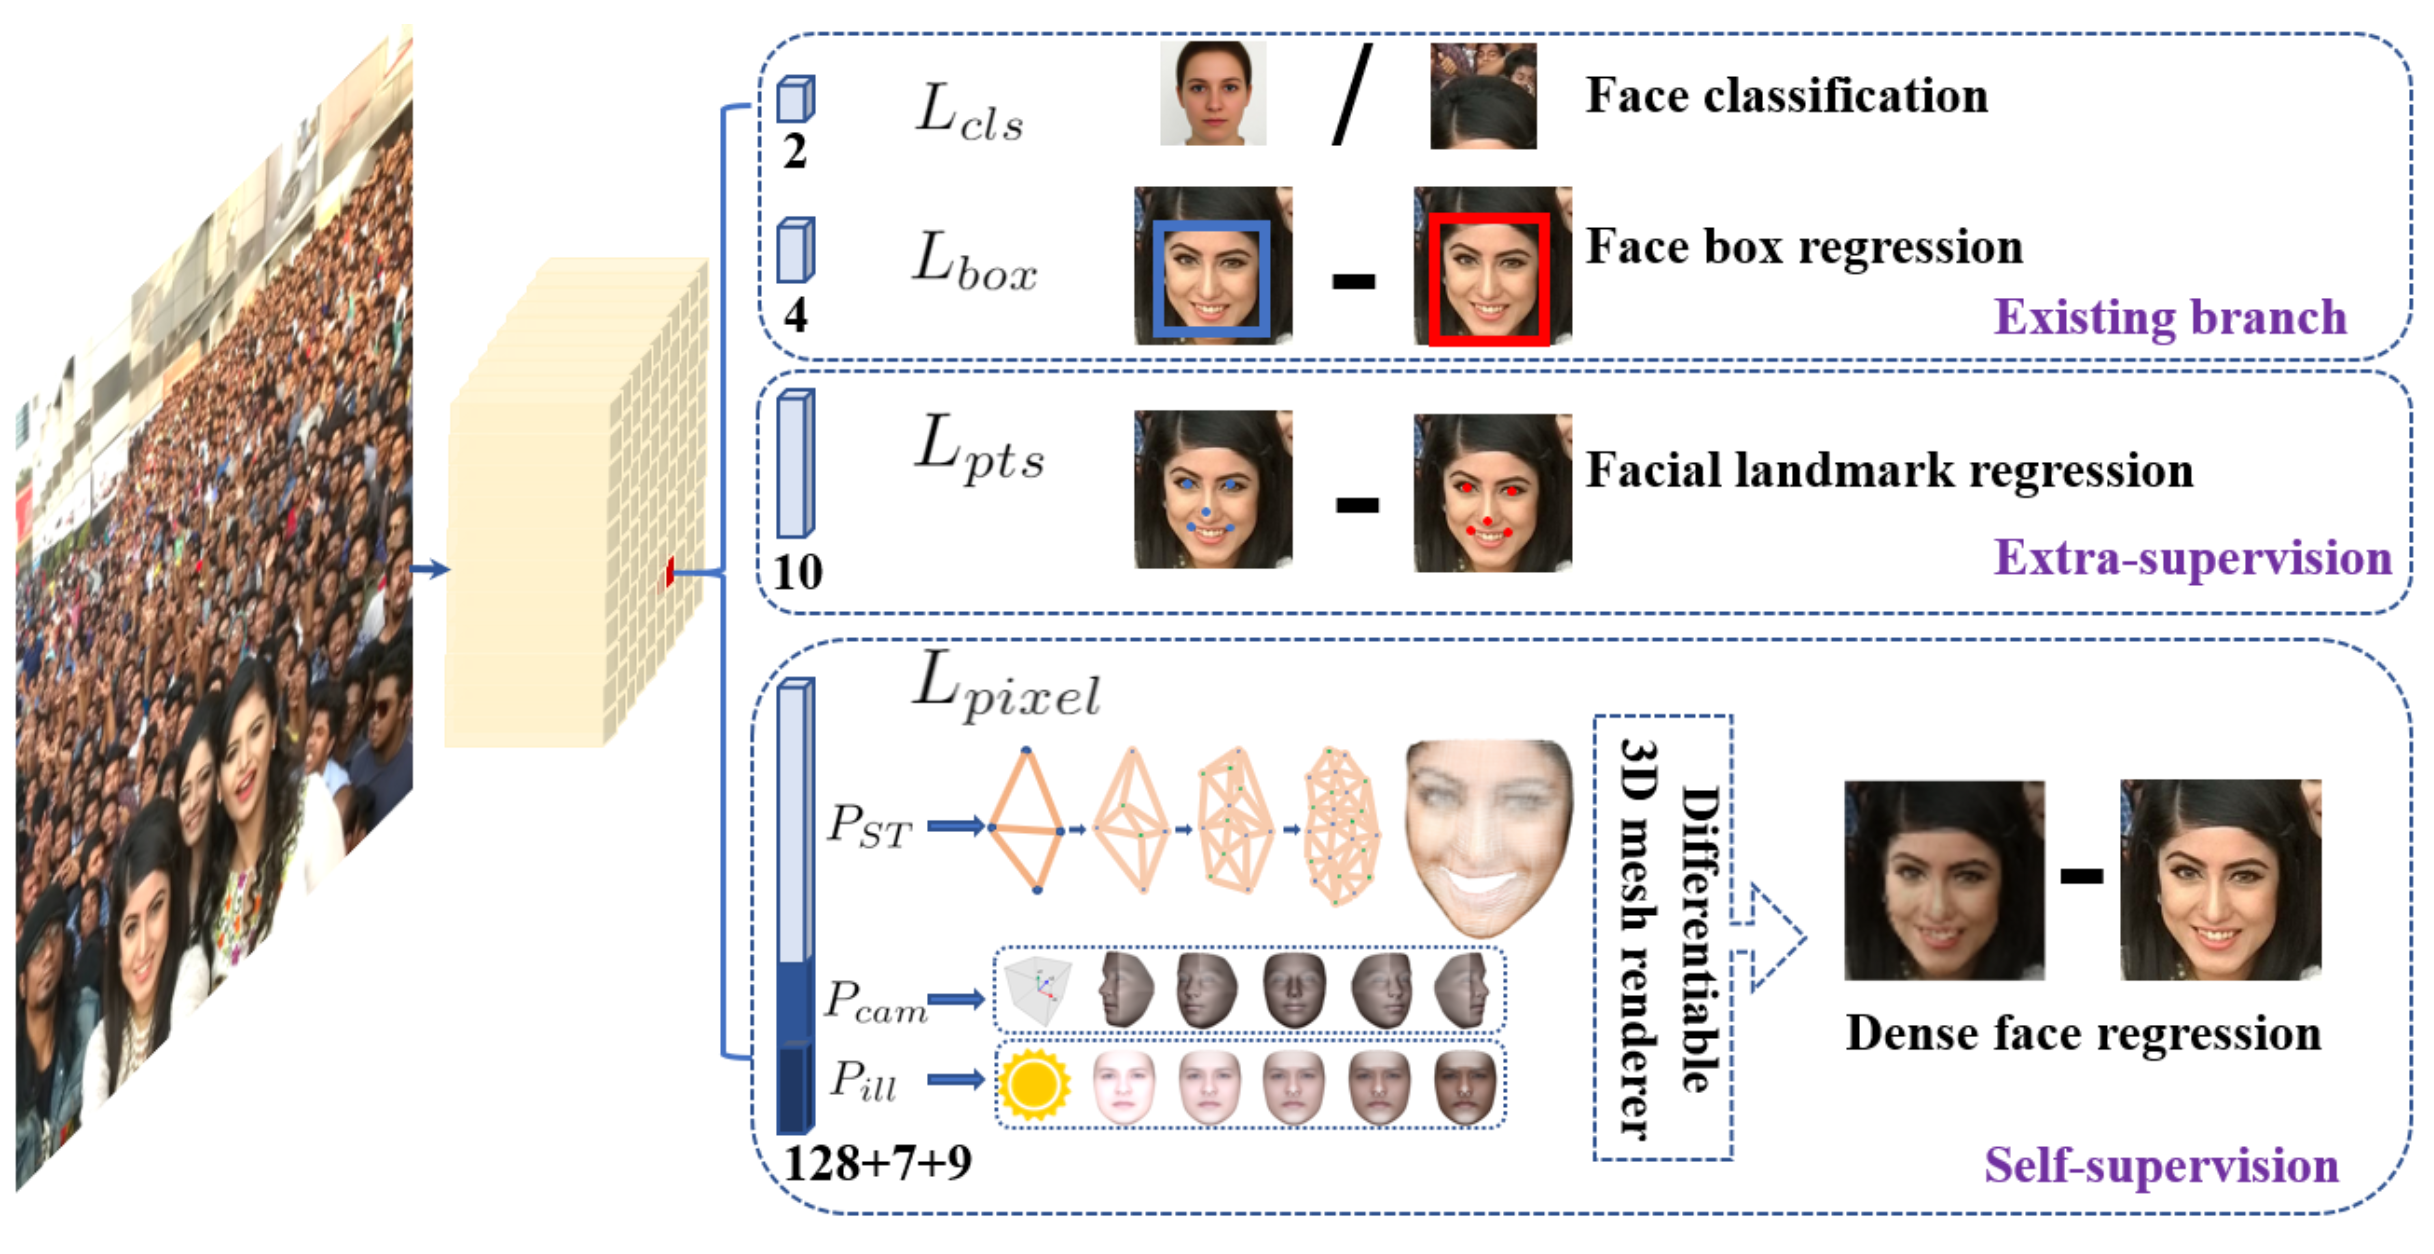
\includegraphics[width=10cm] {images/retinaface_loss_funcs}
        \caption{Ý tưởng các hàm loss multi-task của mô hình RetinaFace. Ngoài hàm loss self-supervision \cite{zhou2019dense, genova2018unsupervised}, các hàm loss còn lại được kế thừa cho mô hình RetinaFocus (Nguồn: \cite{deng2020retinaface})}
        \label{fig:retinaface_loss_funcs}
    \end{figure}

    Cụ thể, trong quá trình huấn luyện mô hình, với mỗi anchor \index{anchor}, nhánh Detection \index{nhánh Detection} của mô hình RetinaFocus tối ưu hàm loss multi-task dưới đây:

    \begin{equation}
        \begin{split}
        L  & =  L_{cls}(p_i, p^{*}_i) + \lambda_1 p^{*}_i L_{box}(t_i, t^{*}_i) + \lambda_2 p^{*}_i L_{pts} (l_i, l^{*}_i).\\
        \end{split}
        \label{eq:retinaface_loss}
    \end{equation}

    \noindent
    trong đó: \\
    - Các trọng số $\lambda_1, \lambda_2, \lambda_3$ được nhóm tác giả cấu hình mặc định là 0.25, 0.1 và 0.01. \\
    - Hàm loss phân lớp mặt: \\
    $L_{cls}(p_i, p^{*}_i)$ với $p_i$ là xác suất mà mô hình dự đoán một anchor \index{anchor} có chứa là khuôn mặt hay không.
    Ta có $p^{*}_i = 1$ nếu anchor \index{anchor} đó chứa khuôn mặt còn $p^{*}_i = 0$ nếu anchor \index{anchor} đó không chứa khuôn là mặt. \\
    - Hàm loss hồi quy định vị vị trí của bbox: \\
    $L_{box}(t_i, t^{*}_i)$ với $t_i=\{t_x, t_y, t_w, t_h\}_i$ và $t^{*}_i=\{t^{*}_x, t^{*}_y, t^{*}_w, t^{*}_h\}_i$ lần lượt là bộ bốn tham số đại diện cho toạ độ của anchor \index{anchor} mà mô hình dự đoán là mặt và bbox ground-truth từ bộ dữ liệu.
    (x là toạ độ x của điểm góc trái trên, y là toạ độ y của điểm góc trái trên, w là chiều rộng của bbox và h là chiều cao của bbox). \\
    - Hàm loss hồi quy định vị vị trí của landmarks: \\
    $L_{pts} (l_i, l^{*}_i)$ với $l_i=\{l_{x_1}, l_{y_1}, \dots , l_{x_5}, l_{y_5}\}_i$ và $l^{*}_i=\{l^{*}_{x_1}, l^{*}_{y_1}, \dots , l^{*}_{x_5}, l^{*}_{y_5}\}_i$ lần lượt là bộ mười tham số đại diện cho toạ độ của năm landmarks mà mô hình dự đoán ứng với mỗi bounding box \index{bounding box} dự đoán và năm ground-truth landmarks của mỗi groundtruth \index{groundtruth} bounding box \index{bounding box} từ bộ dữ liệu.
    
}